\textbf{3.1.} 在铀 $238(^{238}\mathrm{U})$ 的原子核中，两质子间的距离约为 $6.0\times 10^{-15}\mathrm{m}$ 已知质子电荷为 $1.6\times$

$10^{-19}\mathrm{C}$ , 问它们之间的电势能有多少？相互作用的库仑力有多大？

\vfill

\textbf{3.2.} 三个点电荷,其所带电量及位置如习题3.2图所示,计算:

(1) 各对电荷之间的相互作用能；

(2) 电荷系统的相互作用能.
\begin{center}
    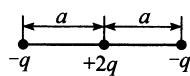
\includegraphics[width=0.2\linewidth]{figures/fig_3_2.jpg}
\end{center}

\vfill

\newpage

\textbf{3.3.} 在边长为 $a$ 的正六边形各顶点有固定的点电荷, 它们的电量交替为 $Q$ 和 $-Q$ , 参见习题 3.3 图.

(1) 求系统的相互作用能；

(2) 若外力将其中相邻的两个点电荷缓慢地移到无限远处, 在移动过程中维持这两个点电荷的距离以及其余电荷的位置不变, 问外力需做多少功?

\begin{center}
    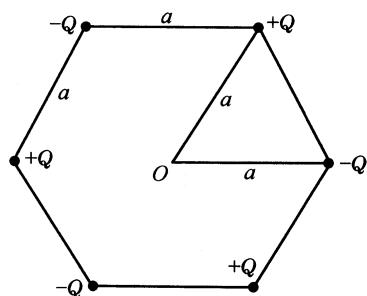
\includegraphics[width=0.2\linewidth]{figures/fig_3_4.jpg}
\end{center}

\vfill

\textbf{3.4.} 假定电子是球形的,并且它的静止能量 $mc^{2}$ (m 是它的静质量,c 是真空中光速)就是来自它的静电能量,这样就可以由它的电荷分布算出它的半径来.
(1) 假定电子电荷 e 均匀分布在球面上, 求电子的半径;

(2) 假定电子电荷 e 均匀分布在球体内, 求电子的半径;

(3) 由于假定电荷分布情况不同, 算出的电子半径便稍有不同. 目前把 $r_0 = e^2 / (4\pi \varepsilon_0 mc^2)$ 称作电子的经典半径. 已知电子电荷 $e = -1.6 \times 10^{-19} \mathrm{C}$ , 电子的静质量 $m = 9.11 \times 10^{-31} \mathrm{~kg}$ , 光速 $c = 3.0 \times 10^{8} \mathrm{~m} \cdot \mathrm{s}^{-1}$ , 求 $r_0$ 的值.


\vfill

\newpage

\textbf{3.5.} 如习题 3.5 图所示, 半径为 $R_{1}=2.0cm$ 的导体球外套一个与它同心的导体球壳, 壳的内外半径分别为 $R_{2}=4.0cm$ 和 $R_{3}=5.0cm$ , 球与壳间充满空气, 壳外也是空气, 球和壳原来都不带电. 现在使球带电 $3.0\times10^{-8}C$ , 问这个系统储藏了多少电能? 如果用导线把球与壳联在一起, 结果如何?
\begin{center}
    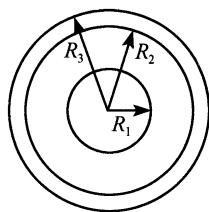
\includegraphics[width=0.2\linewidth]{figures/fig_3_5.jpg}
\end{center}

\vfill

\textbf{3.6.} 铀235原子核可当作半径 $r = 9.2 \times 10^{-15} \mathrm{~m}$ 的球，它有92个质子，每个质子的电荷为 $e = 1.6 \times 10^{-19} \mathrm{C}$ . 假设这些电荷均匀分布在上述球体内.

(1) 求铀 235 原子核的静电势能；

(2) 当一个铀 235 原子核分裂成两个相同的碎片, 每个都可当作均匀带电球时, 求放出的能量;

(3) 1kg 铀 235 裂变时, 能放出多少能量?

\vfill

\newpage

\textbf{3.7.} 半径为 $a$ 的导体圆柱外套有一个半径为 $b$ 的同轴导体圆筒，长度都是 $l$ ，其间充满介电常量为 $\varepsilon$ 的均匀介质，圆柱带电为 $Q$ ，圆筒带电为 $-Q$ ，略去边缘效应.

(1) 在半径为 $r(a < r < b)$ 处，电场能量密度是多少？

(2) 整个介质内的电场总能量 $W$ 是多少？

(3) 试证明： $W = Q^2 / (2C), C$ 是圆柱和圆筒间的电容.

\vfill

\textbf{3.8.} 圆柱形电容器由一根长直导线和套在它外面的共轴导体圆筒构成. 设导线的半径为 $a$ , 圆筒的内半径为 $b$ . 证明: 电容器所存储的能量有一半是在半径为 $r = (ab)^{1/2}$ 的圆柱体内.

\vfill

\newpage

\textbf{3.9.} 由两共轴金属圆柱构成一空气电容器，设空气击穿场强为 $E_{\mathrm{b}}$ ，内外导体圆柱半径为 $R_{1}$ 、 $R_{2}$ ，导体单位长度带电量为 $\lambda_{\mathrm{e}}$ 。在给定 $R_{2}$ 和保证空气介质不致击穿的前提下，应当如何选择 $R_{1}$ ，使得

(1)两导体间的电势差最大?

(2) 电容器的储能最大?

(3) 当空气击穿的场强 $E_{b}=3\times10^{6}V\cdot m^{-1}$ 、 $R_{2}=1cm$ 时，分别计算在(1)和(2)两种选择方案下电容器的极大电势差.

\vfill

\textbf{3.10.} 一球形电容器, 内球壳的外半径为 $R_{1}$ , 带电量为 $Q$ ; 外球壳的内半径为 $R_{2}$ , 带电量为 $-Q$ . 求

(1)二球壳各自的自能, 

(2)二球壳之间的互能, 

(3)系统的总能量.

\vfill

\newpage

\textbf{3.11} 长为 $L$ 的圆柱形电容器由半径为 $a$ 的内芯导线与半径为 $b$ 的外部导体薄壳所组成, 其间填满了介电常量为 $\varepsilon$ 的电介质. 把电容器与电势为 $V$ 的电池相连接, 并将电介质从电容器中拉出一部分. 当不计边缘效应时, 要维持电介质在拉出位置不动, 需施多大的力? 此力沿何方向?


\vfill

\textbf{3.12} 如习题3.12图所示，一平行板电容器的两极板都是长为 $a$ 宽为 $b$ 、面积为 $S = ab$ 的长方形金属片,两片相距为 d, 分别带有电荷 Q 和 -Q. 一块厚为 t、相对介电常量为 $\varepsilon_{r}$ 的均匀介质片(面积和宽度都与极板相同)平行地放在两极板间, 并沿着长度方向部分抽出. 略去边缘效应, 证明: 当介质片在极板间的长度为 x 时, 把它拉向原来位置的静电力为

$$
F = \frac {Q ^ {2} b (d - t ^ {\prime}) t ^ {\prime} d}{2 \varepsilon_ {0} [ S (d - t ^ {\prime}) + x b t ^ {\prime} ] ^ {2}}
$$

式中， $t^{\prime} = (\varepsilon_{\mathrm{r}} - 1)t / \varepsilon_{\mathrm{r}}$

\begin{center}
    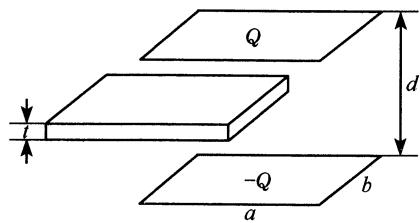
\includegraphics[width=0.3\linewidth]{figures/fig_3_10_1.jpg}
\end{center}
\vfill

\newpage
\textbf{3.13} 如习题 3.13 图所示,一平行板电容器极板的面积为 S, 极板间距离为 d, 在它中间有一块厚为 t、相对介电常量为 $\varepsilon_{r}$ 的介质平板, 把两极板充电到电势差为 V. 略去边缘效应.

(1) 断开电源, 把这介质板抽出, 问抽出时要做多少功?

(2) 如果在不断开电源的情况下抽出, 则要做多少功?

(3) 如果将中间的介质板换上同样厚的导体板, 结果又如何?
\begin{center}
    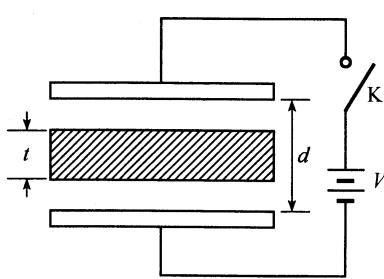
\includegraphics[width=0.3\linewidth]{figures/fig_3_10_2.jpg}
\end{center}
\vfill

\textbf{3.14} 如习题 3.14 图所示, 在接地导体 $z = 0$ 平面的上方 $(x, y, z) = (a, 0, a)$ 和 $(-a, 0, a)$ 处分别有点电荷 $+q$ 和 $-q$ .

(1) 求作用在 +q 上的作用力；

(2) 为了得到这样一个电荷系统, 求反抗静电力所做的功;

(3) 求点 $(a,0,0)$ 处的电荷面密度.
\begin{center}
    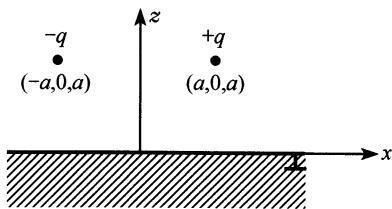
\includegraphics[width=0.3\linewidth]{figures/fig_3_10_3.jpg}
\end{center}
\vfill

\newpage

\textbf{3.15} 一个半径为 $a$ 、带电量为 $q$ 的导体球放入均匀电场 $E_0$ 中，求：

(1) 感应后球的偶极矩；

(2